\documentclass{eceday}

\graphicspath{{./Images/}}
\addbibresource{../References.bib}

\title[Chipyard]{Chipyard: A RISC-V Development Framework}
\subtitle{ECE Day 2021}
\author{Alexander Lukens \and Karl Hallsby \\ Faculty Advisor: Dr.\ Jia Wang}
\institute{Illinois Institute of Technology}
\date{\DTMdisplaydate{2021}{4}{9}{-1}}

\begin{document}

\nocite{chipyard}
\nocite{firesimChipyardOverview}

\begin{frame}
  \titlepage{}
\end{frame}

\section{About Us}\label{sec:About_Us}
\begin{frame}
  \frametitle{\nameref{sec:About_Us}}
  \begin{columns}
    % Alex Picture and Description
    \begin{column}{0.50\linewidth}
      \begin{figure}[h!tbp]
        \centering
        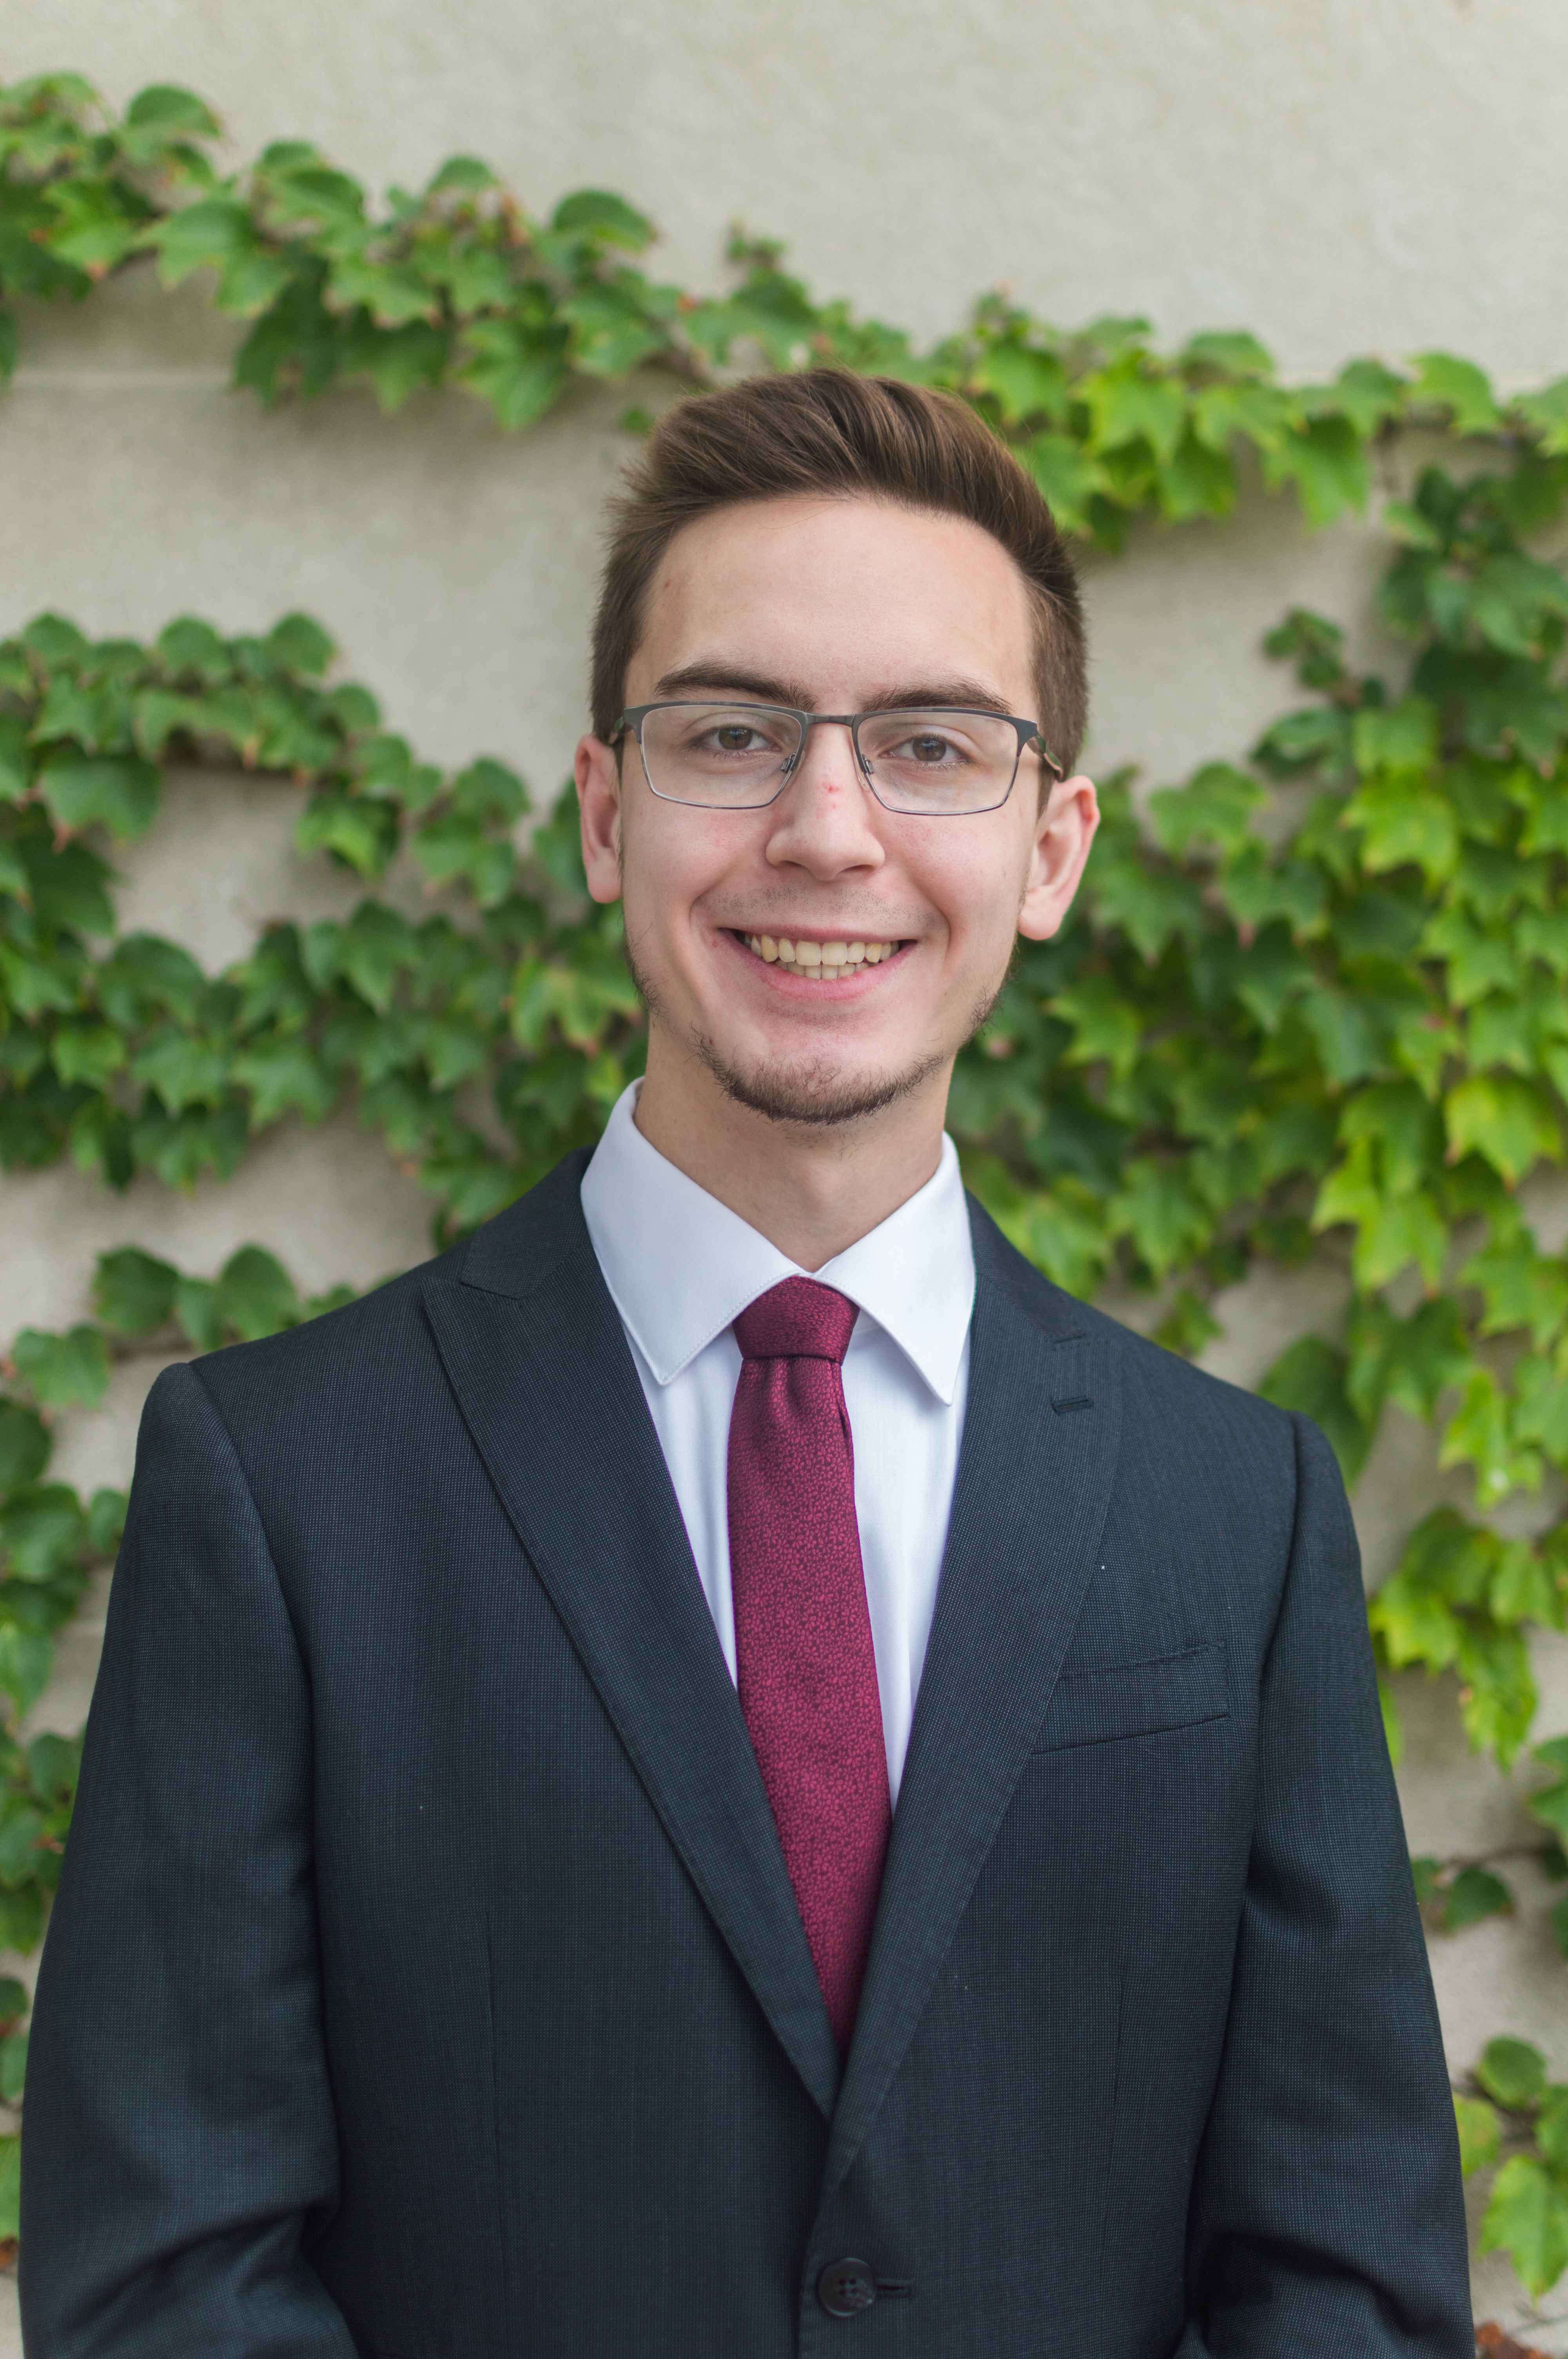
\includegraphics[scale=0.02]{./Lukens_Alex.jpg}
        \caption*{Alexander Lukens}
        \label{fig:Alex_Lukens}
      \end{figure}
  		\begin{center}
          B.S. Electrical Engineering \\
          M.S. Computer Engineering
  		\end{center}
    \end{column}
    % Karl Picture and Description
    \begin{column}{0.50\linewidth}
      \begin{figure}[h!tbp]
        \centering
        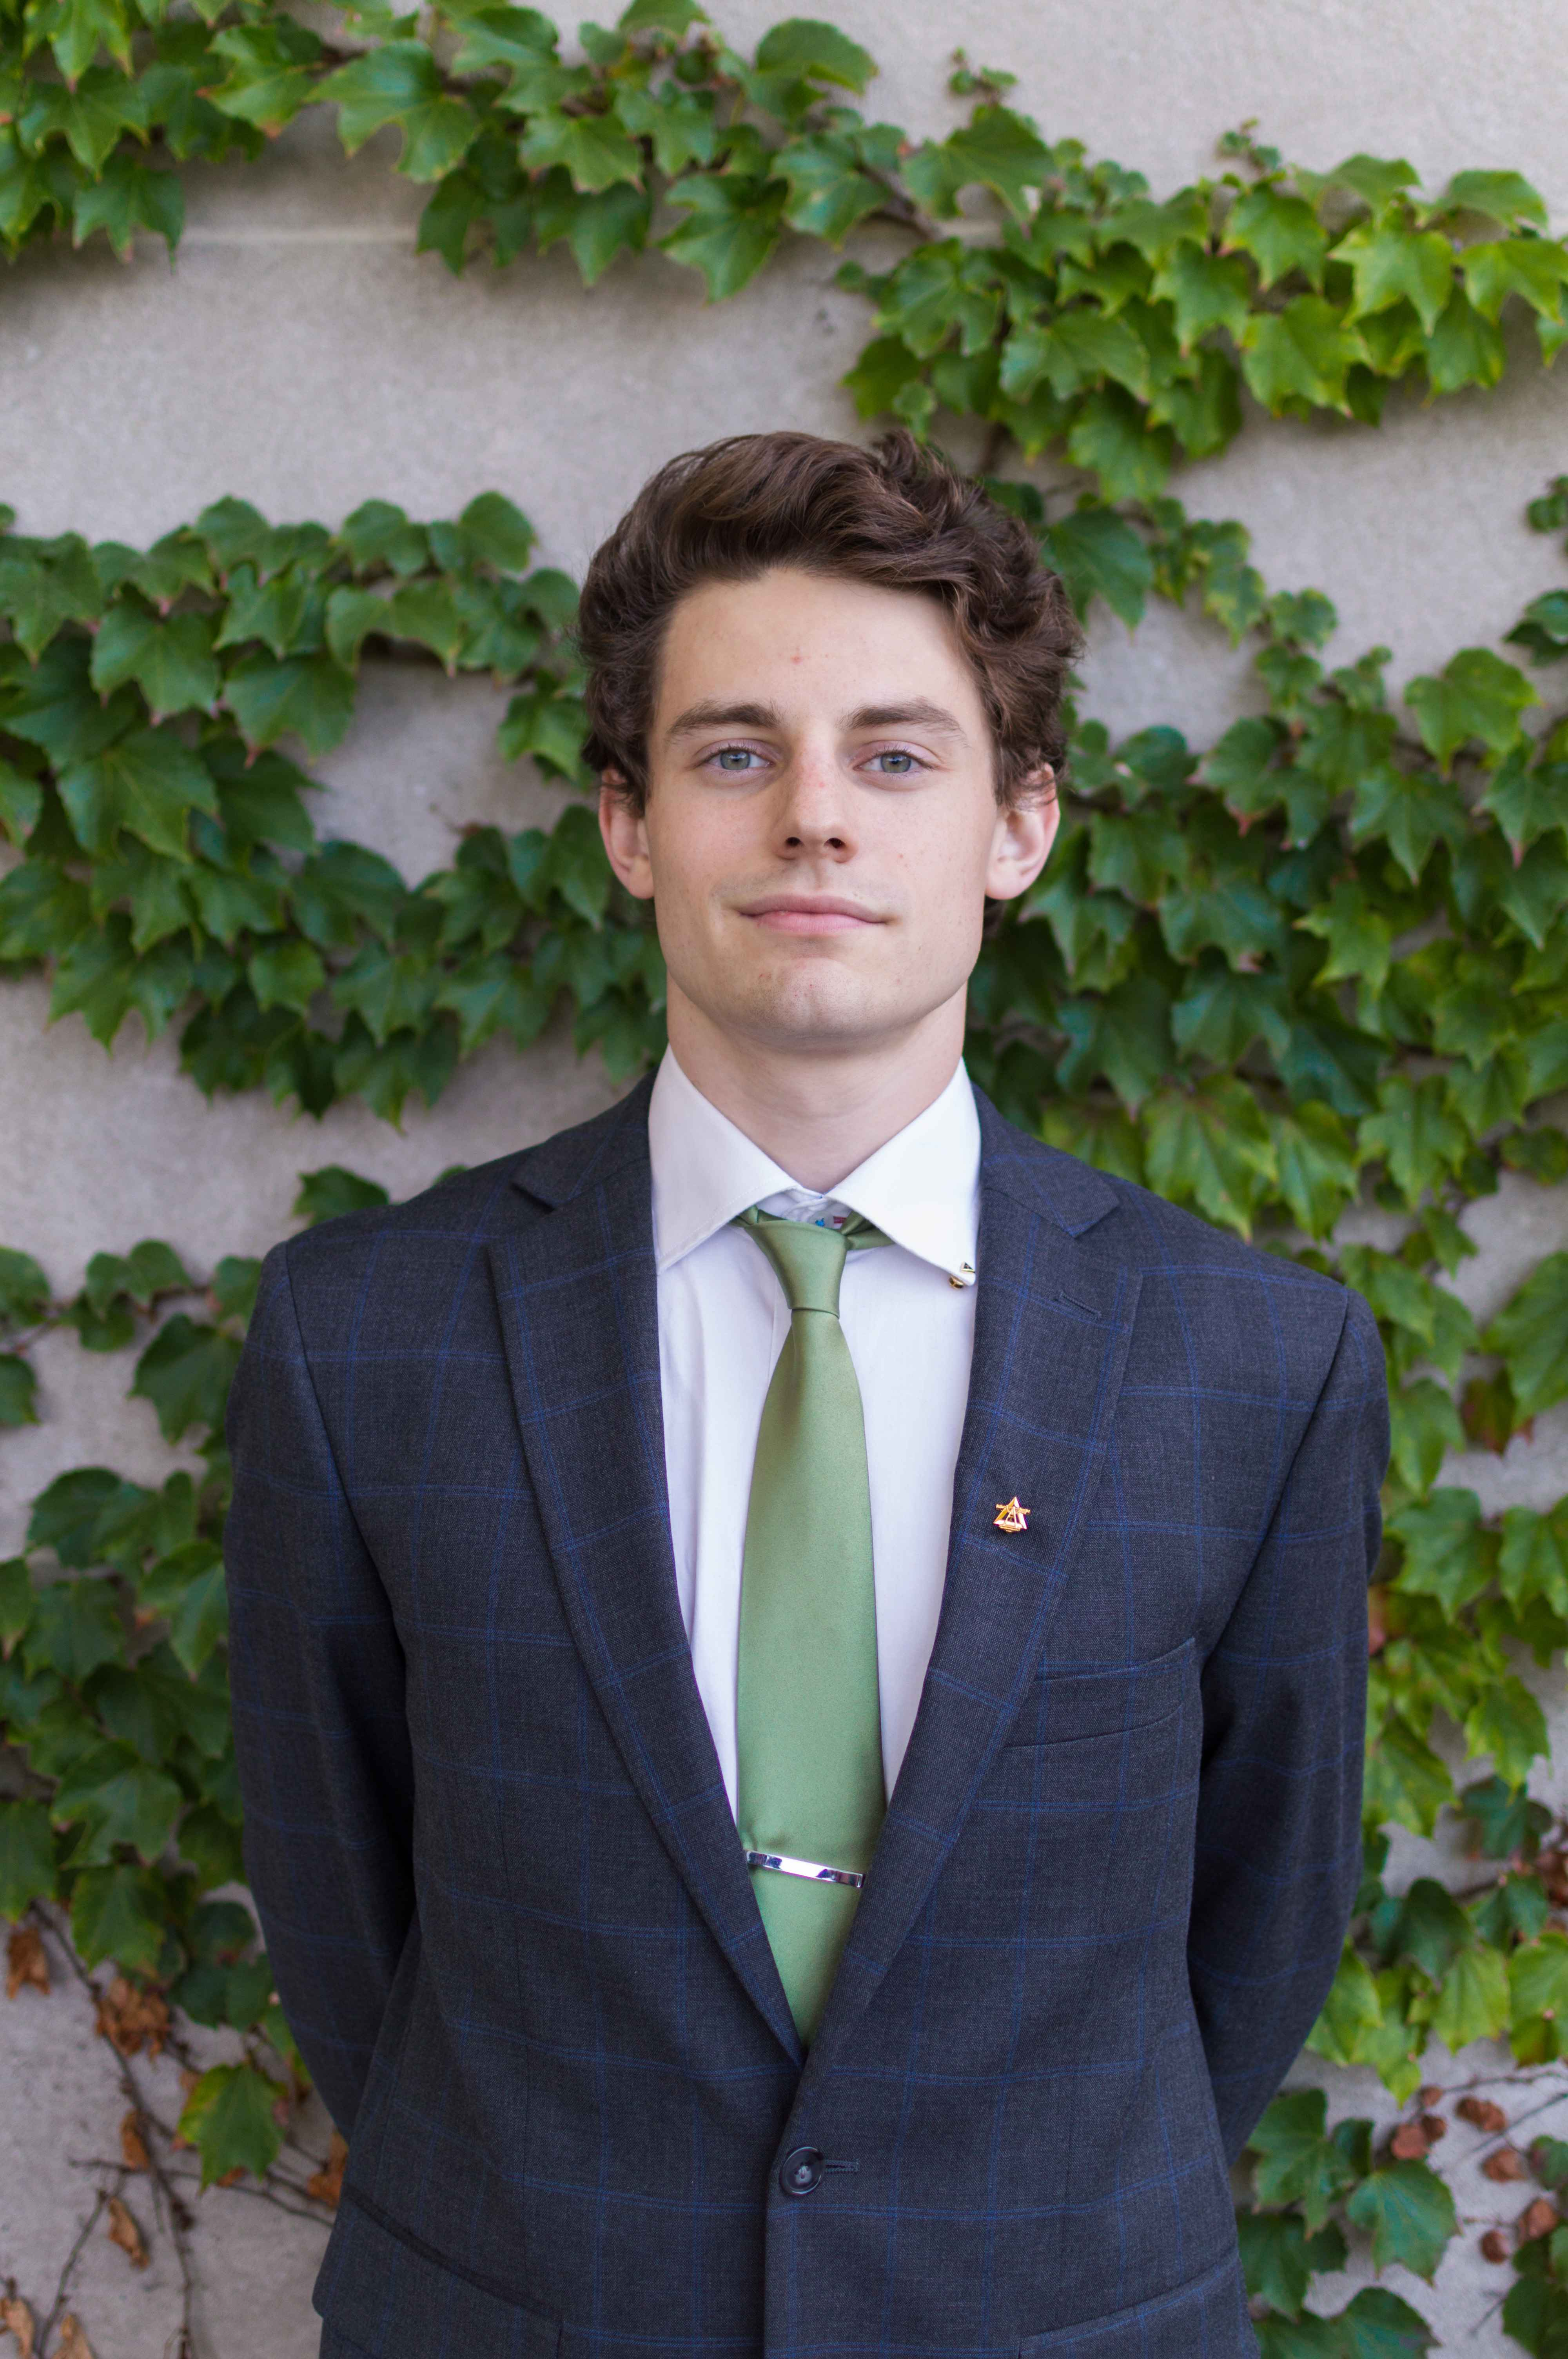
\includegraphics[scale=0.02]{./Hallsby_Karl.jpg}
        \caption*{Karl Hallsby}
        \label{fig:Karl_Hallsby}
      \end{figure}
      \begin{center}
        B.S. Computer Engineering \\
        M.S. Computer Engineering
      \end{center}
    \end{column}
  \end{columns}
\end{frame}

\section{What is RISC-V?}\label{sec:What_is_RISC-V}
\begin{frame}
  \frametitle{\nameref{sec:What_is_RISC-V}}
  \begin{figure}[h!tbp]
    \centering
    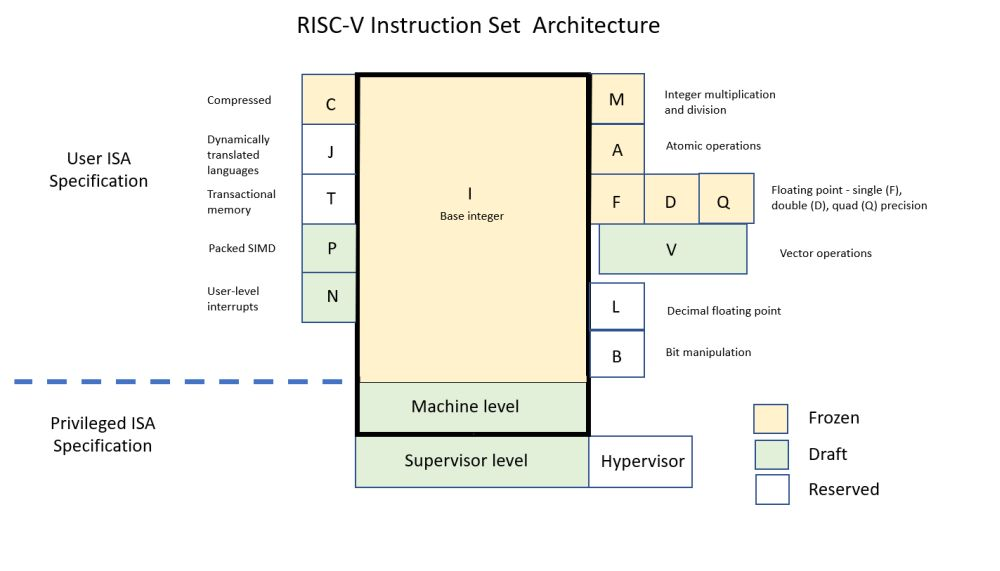
\includegraphics[scale=0.35]{./RISC-V-ISA_and_Extensions.jpg}
    \caption{RISC-V ISA and Standard Extensions \parencite{customRISCVProcessor}}
    \label{fig:RISC-V_ISA-Standard_Extensions}
  \end{figure}
  \vspace{-1.5em}
  \begin{itemize}
  	\item Suitable for use in applications ranging from microcontrollers to supercomputers
  	\item Goal \textrightarrow{} become the industry standard ISA \parencite{FireSimTalk1}.
  \end{itemize}
\end{frame}

\section{What is Chipyard?}\label{sec:What_is_Chipyard}
% Image of silicon they've taped out using Chipyard and its associated tools
\begin{frame}
  \frametitle{\nameref{sec:What_is_Chipyard}}
  \begin{figure}[h!tbp]
    \centering
    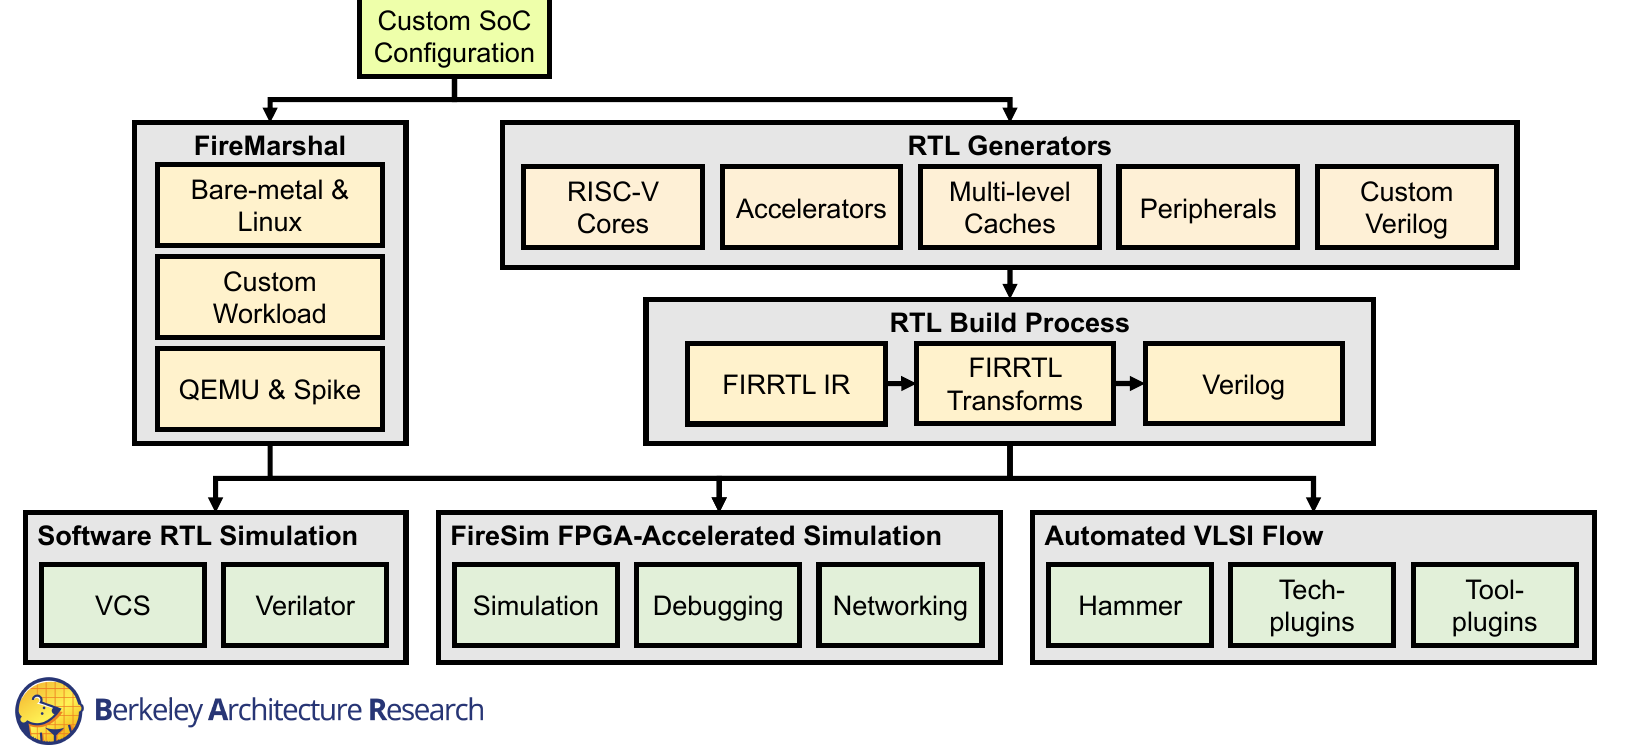
\includegraphics[scale=0.25]{./BAR-Chipyard.png}
    \caption{Chipyard Subcomponents \parencite[p.~3]{firesimChipyardOverview}}
    \label{fig:Chipyard_Subcomponents}
  \end{figure}
  \vspace{-1.5em}
  \begin{itemize}
  \item A framework for generating and testing RISC-V CPUs
  \item Elaborate CPUs using declarative Scala which generates appropriate Verilog
    \begin{itemize}
    \item Can also generate FPGA bitstreams, \texttt{mcs} files, and other data formats
    \end{itemize}
  \end{itemize}
\end{frame}

\section{What We Did}\label{sec:What_We_Did}
\begin{frame}
  \frametitle{What We Did}
  \begin{itemize}
  \item Explore repository to more fully understand how everything works together
  \item Build standard CPUs, already defined in Chipyard
  \item Create configurations to generate custom CPUs
  \item Write standard CPUs out to FPGAs for testing
    \begin{itemize}
    \item Identified issues with Chipyard's implementation of Arty FPGA support
    \end{itemize}
  \item Upload programs to built FPGA CPU
  \end{itemize}
\end{frame}

\section{What We Learned}\label{sec:What_We_Learned}
\begin{frame}
  \frametitle{\nameref{sec:What_We_Learned}}
  % TODO: Include the challenges we faced while working on this project here
  \begin{itemize}
  \item Chipyard is under active development
    \begin{itemize}
    \item Some components are not fully implemented, or not supported at all
    \item Codebase is still fluctuating in usability, the FPGA design flow does not include support for all peripherals yet
    
    \end{itemize}
  \item The Verilog simulation of RISC-V processors in Chipyard is very robust, allows for comprehensive testing of a design to ensure ISA compliance
  \end{itemize}
\end{frame}

\section{Next Steps}\label{sec:Next_Steps}
\subsection{Educational Laboratory Work}\label{subsec:Educational_Lab_Work}
\begin{frame}
  \frametitle{\nameref{subsec:Educational_Lab_Work}}
  \begin{itemize}
  \item Open nature of RISC-V allows for easy, license-free tinkering of CPU designs
  \item Strong documentation of RISC-V architectures due to industry use
  \item Open development allows for easy tracking of changes made to underlying CPU designs
  \item Other universities already use Chipyard and RISC-V for undergraduate computer architecture courses
  \end{itemize}
\end{frame}

\subsection{Further Research Work}\label{subsec:Further_Research_Work}
\begin{frame}
  \frametitle{\nameref{subsec:Further_Research_Work}}
  \begin{itemize}
  	\item Increase compatability with components on Arty FPGA board
  	\item GPIO, Ethernet, LEDs, Switches, external devices, etc.
  	\item Design and integrate GPIO device that will assist with debugging (single-step bus cycle, display current memory address, program counter, register contents)
  	\item Investigate VLSI Design flow in Chipyard

  \end{itemize}
\end{frame}

\section{Conclusion/Deliverables}\label{sec:Conclusion_Deliverables}
% The Book and our documentation
\begin{frame}
  \frametitle{\nameref{sec:Conclusion_Deliverables}}
  \begin{itemize}
  \item Chipyard offers many tools that greatly enhance the development of larger RISC-V CPU designs
  \item We are preparing a documentation manual covering everything we did. This includes:
    \begin{itemize}
    \item Environment Setup \& Configuration
    \item Basic Steps for Generating a first CPU
    \item A walkthrough of the Chipyard repository's structure
    \item A discussion on how to write FPGA images out and use them for testing
    \end{itemize}
  \end{itemize}
\end{frame}

\section{Demonstration}\label{sec:Demonstration}
\begin{frame}
  \vfill
  \centering
  \begin{beamercolorbox}[sep=8pt,center,shadow=true,rounded=true]{title}
    \usebeamerfont{title}\nameref{sec:Demonstration}\par%
  \end{beamercolorbox}
  \vfill
\end{frame}

\begin{frame}
  \frametitle{References}
  \printbibliography[heading=bibintoc]{}
\end{frame}

\end{document}

%%% Local Variables:
%%% mode: latex
%%% TeX-master: t
%%% End:
